%!TEX root = ../report.tex


%%%%%%%%%%%%%%%%%%%%%%%%%%%%%%%%%%%%%%%%%%%%%%
\chapter{Delanalyse 2: Forskelle i sociale processer \label{kapitel_delanalyse2_socialeprocesser}}
%%%%%%%%%%%%%%%%%%%%%%%%%%%%%%%%%%%%%%%%%%%%%%

Lorem ipsum dolor sit amet, consectetur adipisicing elit, sed do eiusmod
tempor incididunt ut labore et dolore magna aliqua. Ut enim ad minim veniam,
quis nostrud exercitation ullamco laboris nisi ut aliquip ex ea commodo
consequat. Duis aute irure dolor in reprehenderit in voluptate velit esse
cillum dolore eu fugiat nulla pariatur. Excepteur sint occaecat cupidatat non
proident, sunt in culpa qui officia deserunt mollit anim id est laborum.

%%%%%%%%%%%%%%%%%%%%%%%%%%%%%%%%%%%%%%%%%%%%%%
\section{Indkomst og arbejde \label{sec_delanalyse2_loen}}
%%%%%%%%%%%%%%%%%%%%%%%%%%%%%%%%%%%%%%%%%%%%%%

Når man undersøger sit eget forslag til arbejdsmarkedsstruktur skal man være opmærksom på, at det ikke kan valideres med ved hvad Boje kalder “outcomes af sociale processer,” såsom arbejdsløshed, hyppighed i jobskift og, ikke mindst: lønforskelle \parencite[28]{Boje1985}. Det er indkomst og indkomstforskelle mellem delmarkederne, jeg vil gennemgå nu. 

I netværksmetodologiske termer er Laumann, Marsden \& Prensky inde på det samme, når de advarer imod at validere et socialt netværk baseret på de selvsamme attributter, der er brugt til at konstruere det \parencite[29]{Laumann1983}. Løn er ikke brugt til at konstruere mit netværk, men må siges at være så tæt et outcome af beskæftigelse, at det ikke fremstår eksternt i Lauman et als (skriver man det sådan? \#todo) forstand. Lønniveauerne på de af Moneca skabte \emph{delmarkeder} er derimod interessante for validiteten, hvis vi accepterer det som et \emph{kriterie-relateret validitetsmål}, der gør det muligt at validere den interne struktur og konsistens i et klasseskema \parencite[94]{Oesch2006a}%
%
\footnote{ Jeg laver ikke et klasseskema, men er tæt nok på til jeg synes det giver mening at benytte Oeschs validitetskriterie.}%
%
. Udover denne mere metologisk nødvendige validering af mit bud på en segmenteringsstrukur, er lønninger \emph{i sig selv} interessante, da det er direkte relaterbart til arbejdsmarkedets struktur, og utvivlsomt er den mest benyttede indikator for social status og magtposition i den sociale struktur Oesch s. 95, (Weber, Andrade, Boje, Marx, Wright, Goldthorpe, Harrits, Scott - find dem og skriv dem ind \#todo.) 

Jeg benytter indkomstvariablen timeløn. I bilag \ref{app_loen} beskriver jeg variablen samt den datarensning jeg foretager, samt sammenligner den med de andre mulige indkomstvariable og DSTs egne mål for indkomst for forskellige erhvervsgrupper. De væsentlige pointer fra bilaget er:

 %
 \begin{itemize}
  \itemsep -0.5em
  	\item Timelønsvariablen er det bedste skøn på indkomst, og er ganske nøjagtigt selv på mit detaljerede \texttt{DISCO}-niveau.
  	\item Medmindre andet siges, er timelønninger \emph{et gennemsnit} af lønningerne i hele perioden 1996-2009. I beregningen af dette gennemsnit er perioden 1996-2008 inflationskorrigeret til 2009 priser.
  	\item Månedslønninger beregnes ved at gange timelønnen med 160,33. Det er DSTs metode \parencite[32]{DST2009}.
 \end{itemize}
%


%
\subsection{Timelønninger for delmarkederne \label{subsec_delanalyse2_loenninger}}
%

Indkomstfordelingen i den arbejdende del af den danske befolkning kan ses i  \ref{delanalyse2_timelon_fordelingogfigur}. 

Vi kan se at indkomstfordelingen er nogenlunde centreret omkring gennemsnittet og medianen, hvilket også kommer til udtryk i standardafvigelsen på 76 kr/t. Det ses at fra > 250 kr/t falder antallet af personer ganske drastisk, hvilket også kan aflæses i percentilerne. Den “lange hale” af meget høje lønninger er ikke mange forundt, men det er tydeligt, at de, der så tjener over den 90. percentil, tjener eksponentielt mere og mere frem mod den højest (beregnede) timeløn på 2.155 kr. Det lave antal observationer skyldes at dette ikke er beregnet ud fra \texttt{DISCO}-grupperne, men ud fra antallet af personer: Det vil sige, at gennemsnittet er afhængigt af om vedkommende har været på arbejds


\begin{figure}
\parbox[H]{8cm}{\null
  % \centering
  \captionof{figure}{indkomstfordeling i analyseudvalget, farvelagt efter udvalgte percentiler}
	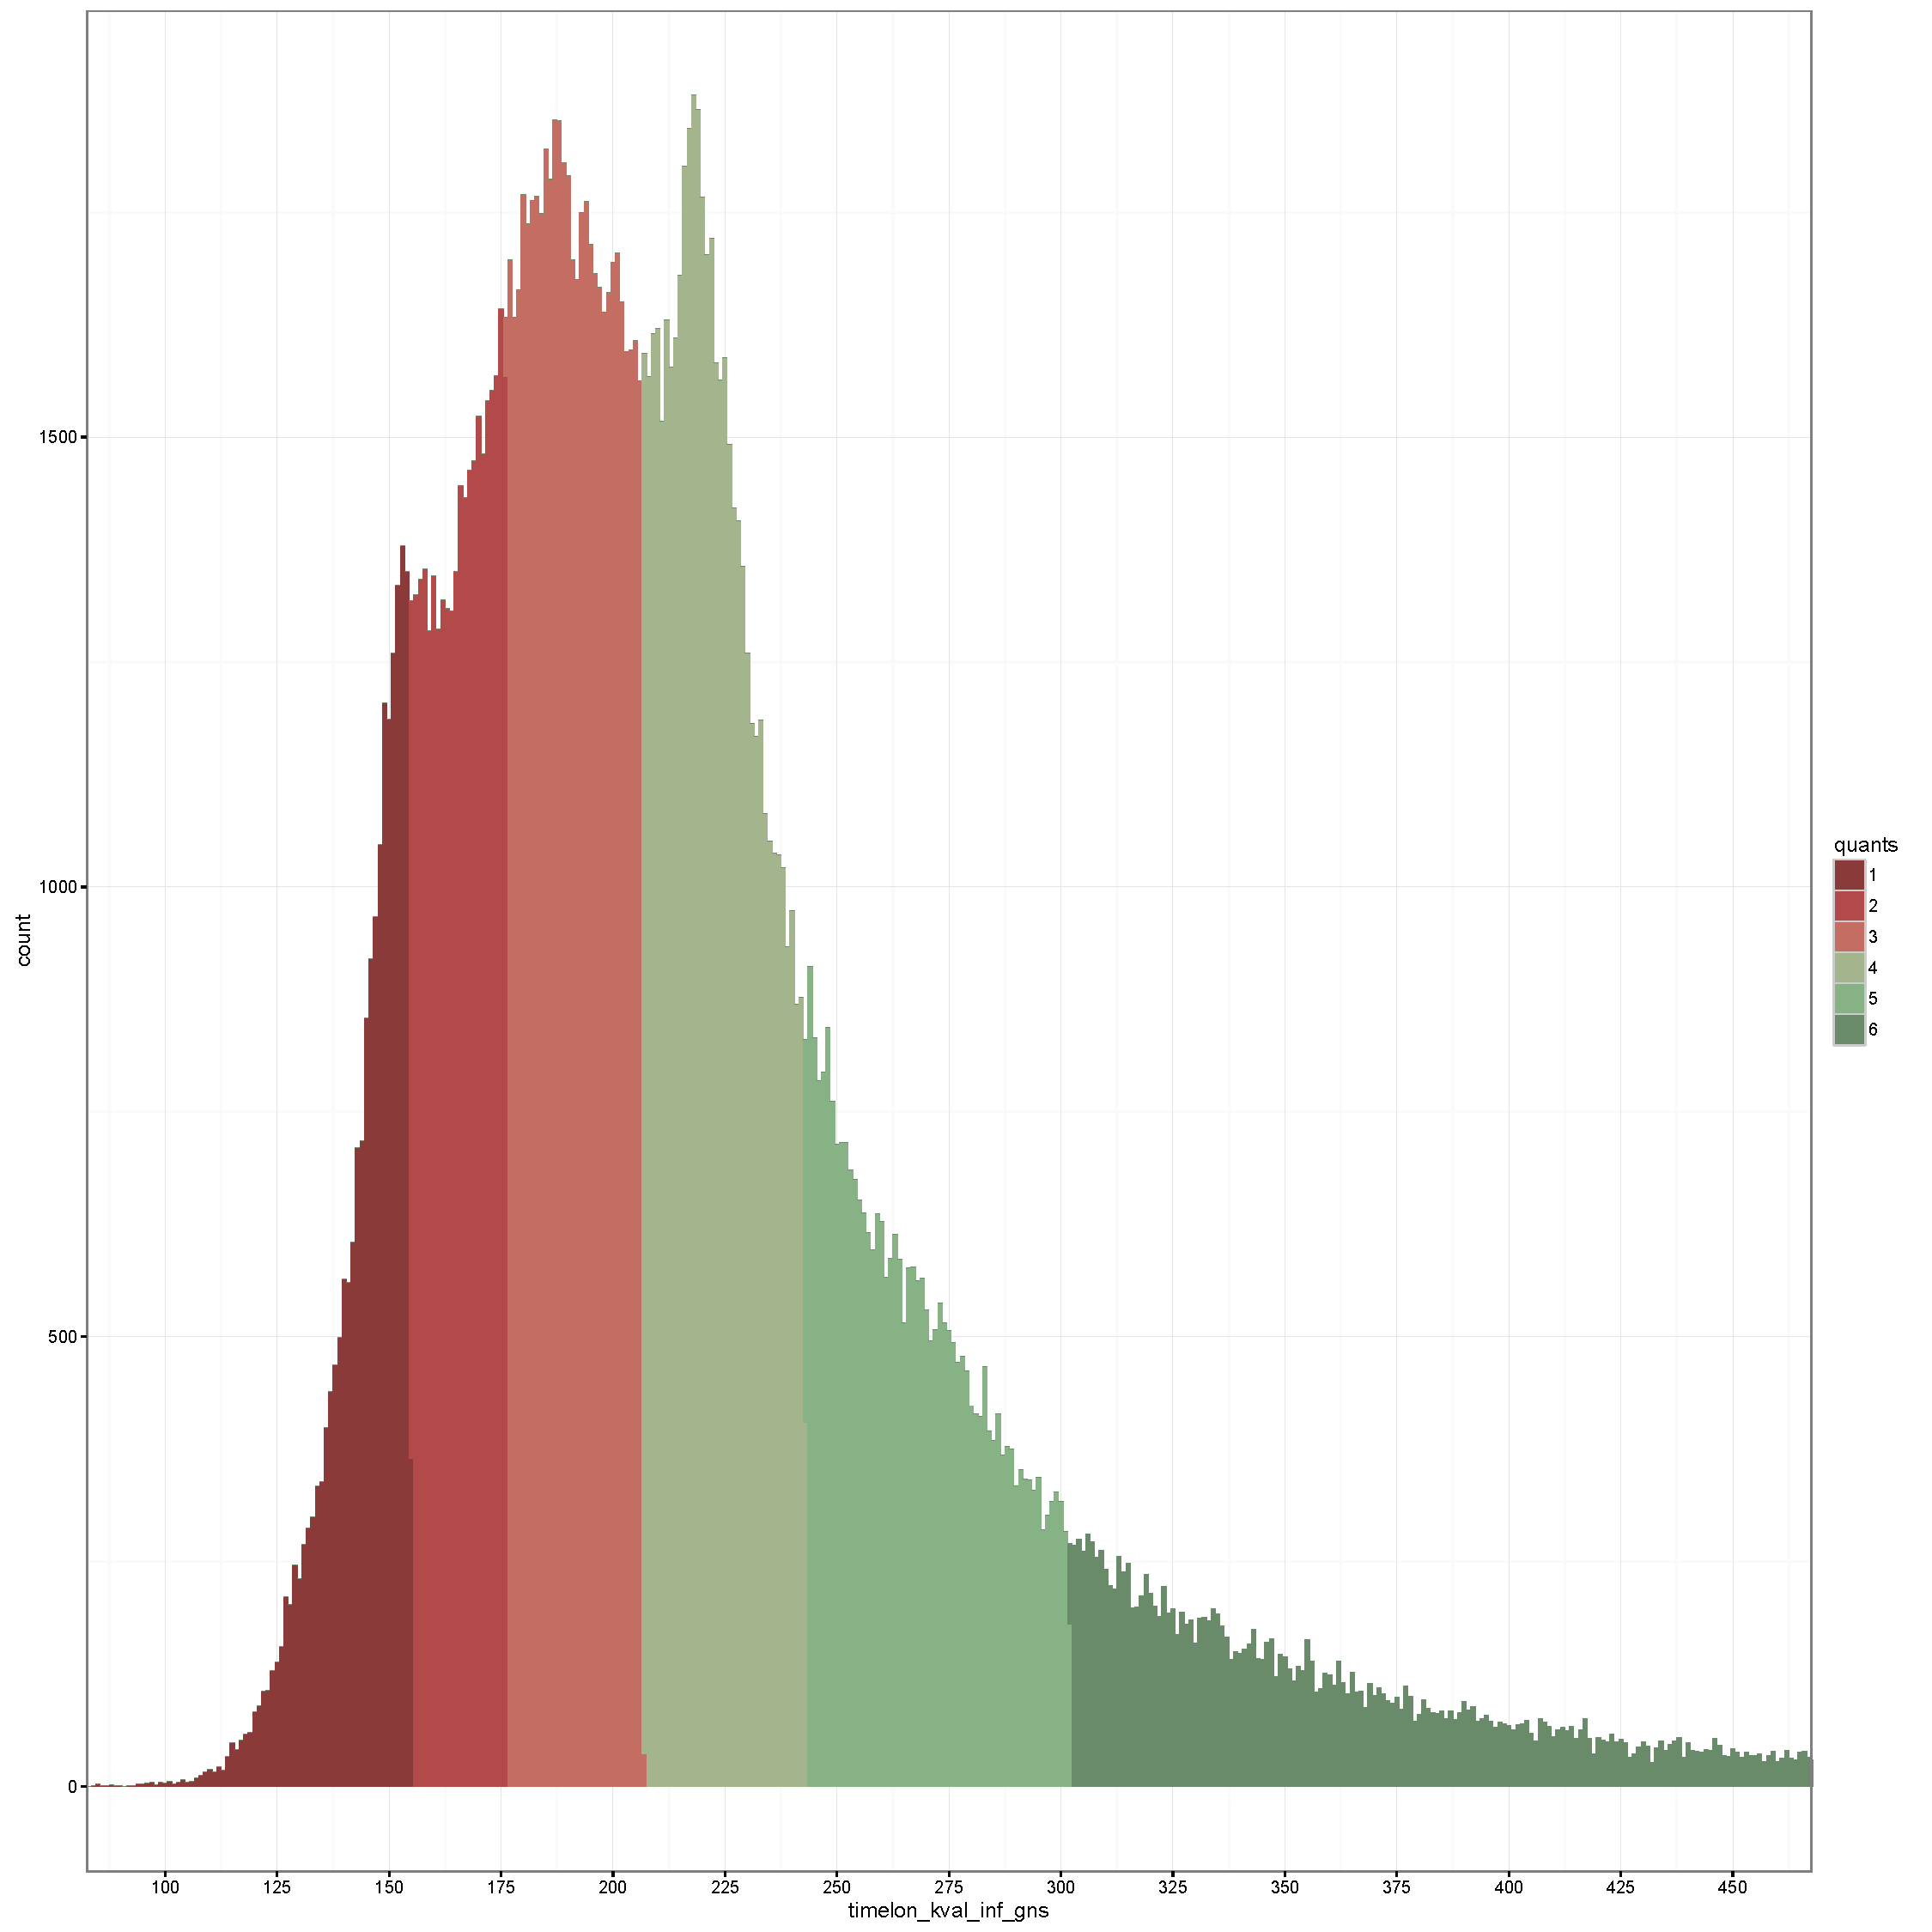
\includegraphics[width=7cm]{fig/deskriptive/timelon_quants.pdf}
}
\parbox[H]{5cm}{\null
\centering
  % \vskip-\abovecaptionskip
  \captionof{table}[t]{Udvalgte mål for indkomstfordelingen \label{delanalyse2_timelon_fordelingogfigur}}%
  \vskip\abovecaptionskip
%
% Table generated by Excel2LaTeX from sheet 'delanalyse2_indkomstfordeling'
\begin{tabular}{lr}
\toprule
Gennemsnit &                    222 kr.  \\
Sd-afvigelse &                      76 kr.  \\
\midrule
Mindste værdi &                      18 kr.  \\
Højeste værdi &                 2.155 kr.  \\
\midrule
10. percentil &                    155 kr.  \\
25. percentil &                    177 kr.  \\
Median &                    207 kr.  \\
75. percentil &                    243 kr.  \\
90. percentil &                    302 kr.  \\
\midrule
\textit{n} & \textit{205.798} \\
\bottomrule
\end{tabular}%

%
}
\end{figure}
%



Vi skal nu kigge nærmere på differentieringen i timeløn, og se, om de i kapitel \ref{delanalyse1_segmenteringsprocessen} fundne delmarkeder kan fortælle os noget om løndiffentieringener på arbejdsmarkedet. Hvem ved? Jeg gør ihvertfald ikke! Vi finder ud af det hen af vejen, det bliver superspændende!









\iffalse
\label{iffalse}
















Attributterne er ikke anvendt som inklusionskriterier og kan derfor bruges til at
vurdere, hvorvidt der er overensstemmelse mellem privilegerede positioner i netvær-
ket og symbolske eller økonomiske privilegier, der er eksterne for netværket. Dette giver
os mulighed for at vurdere om vores specifikation af netværket stemmer overens med
magtsymboler, hvilket kan benyttes til at vurdere validitet ( 1983, s. 29).


validitet i et klasseskema: ekstern og intern validitet (Oesch s. 94)

indkomst som udtryk for magt på arbejdsmarkedet og social status. Dermed "den afgørende faktor" for menneskers livschancer. s. 95

Boje peger på faren ved at fokusere på outcomet af sociale processer såsom lønforskelle, arbejdsløshed, hyppige jobskifte m.m.. Det er en reel fare ved mit empiriske arbejde. s. 28, men meget god hvis man vil sikre sig at alt er, som det skal være. 

Grundet den danske struktur og fokus på organisering må det forventes, at mobilitets- og lønbarrierer primært findes indenfor fag, og ikke indenfor industrier/erhvervsgrene, hvilket findes i USAs langt mindre organiserede og mere monopolitiske virksomhedskultur. 

"i perioder med økonomisk tilbagegang og hvor der på arbejsmarkedet er overudbud af lønarbejdere synes barriererne mellem segmenterne at blive skærpet." (...) og nye segmenter og delmarkeder opstår på den baggrund. s. 72
→ perioden 1996-2009 er en periode med vækst, dvs: Det her en god periode. Find tal for økonomisk vækst for perioden


brug relative forskel mellem lønninger, ikke bare den absolutte, som må siges at være den vigtigste for personerne selv. Brug medianen for den "nederste klasse" som udtryk for lønniveauet. Kan du overføre det til dit eget? lønniveauet for den lavest tjenende klynge?

Oesch afviser at "future prospects" skulle have stor betydning, da han mener at påvise en stærk sammenhæng mellem nuværende lønninger og fremtid indkomst. I danmark, viser Esping-Andersen, fungerer low-income jobs sådan. Men vi kan jo se, hvor folk bevæger sig hen. Og det ser ikke ud til at være en stærk sammenhæng mellem service-jobs og future prospects. Undersøg servicejobs og ande


find ud af hvor mange skift der er per år. Dejligt konkret tal. henvis til boje 1988 s. 123




Løndannelsen s. 79-80
	i det sekundære arbejdsmarked synes der ikke at være en sammenhæng mellem løn og uddannelse - det er ikke det, der er det centrale. Hvorimod på det primære arbejdsmarked synes det netop at være betydningsfuldt, her er uddannelsesmæssige ressource nøje afstemt med løn. 
	tre forhold spiller ind:
	- institutionel regulering kontra markedsregulering: I DK er stort set al løndannelse reguleret gennem institutionelle aftaler 
	→ har nok ændret sig noget siden, men i det store og hele nok stadig rigtigt
	- Lønnen knyttet til job kontra til præstation.
	- lønnen tilnyttet stillingsmæssigt avancement/ikkeavancement. primære forskel på sekundær/primær løn. det sekundære jobmarked har samme lønninger livet igennem. 





















% %%%%%%%%%%%%%%%%%%%%%%%%%%%%%%%%%%%%%%%%%%%%%%
% \section{kønsforskelle i sociale processer \label{sec_delanalyse2_køn}}
% %%%%%%%%%%%%%%%%%%%%%%%%%%%%%%%%%%%%%%%%%%%%%%

% En grundlæggende differentieringsform i snart sagt alle samfund er



%  kønsopdelingen, der kommer til udtryk i en kønsbestemt arbejdsdeling i langt de fleste samfund. Som David Oesch bemærker, er det påfaldende, hvor få kvantitative undersøgelser af arbejdsmarkedsrelationer, der inddrager køn i analyserne  














\fi


